\documentclass[slidetop, mathserif]{beamer}

% \mode<presentation>
% {
% 	\usetheme{Warsaw}
% 	\setbeamercovered{transparent}
% }

% \usepackage{caption}
\usepackage{subcaption}
\captionsetup{compatibility=false}


\mode<presentation>{
	\usetheme{Berlin}
	\setbeamercovered{transparent}
	\usefonttheme{professionalfonts}
}

\usepackage{amsmath, amsfonts, amssymb}
\usepackage{mathrsfs,dsfont}

\newcommand{\norm}[1]{\left\|#1\right\|}
\newcommand{\suchthat}{-\hspace{-10pt}\ni\hspace{-10pt}-}


\AtBeginSection[]
{
   \begin{frame}
       \tableofcontents[currentsection]
   \end{frame}
}

\addtobeamertemplate{navigation symbols}{}{%
    \usebeamerfont{footline}%
    \usebeamercolor[fg]{footline}%
    \hspace{1em}%
    \insertframenumber/\inserttotalframenumber
}

%% want to use verbatim: \begin{frame}[fragile]

\title[Metrics for Tracking]{Metrics for Evaluating Trackers}
\author[chy1010]{Chien, Hung-Yu \\ {\small\tt hungyu@linkernetworks.com}}
\date{\today}

\begin{document}

\begin{frame}
	\titlepage
\end{frame}

\section[Outline]{}
\begin{frame}
	\frametitle{Outlines}
	\tableofcontents
\end{frame}


\begin{frame}
	\frametitle{What is a tracker?}

	A {\bf tracker} is a \emph{model} or a \emph{post-processor}
	that performs on a video, i.e. a sequence of image frames.

	\quad

	A tracker model is often used on MOT (multiple object tracking) tasks,
	which consists of
	\begin{itemize}
	\item to detects objects inside each frames, and
	\item
		to recognizes if the detections in consecutive frames are the
		same or not.
	\end{itemize}

	\quad

	We also use the term `tracker' to indicate the recognization part
	in particular. In this case, trackers are often seem as post-processors
	in model pipelines.

\end{frame}


\section{Trackers and Multiple Object Tracking}

\begin{frame}
	\frametitle{Inference Results of a Tracker}

	Unlike SOT (single object tracking), MOT are mainly to deal with
	multiple objects of the same category. And a tracker should assign
	an identity to each detected object along a video file or a video
	stream.

	\begin{figure}
		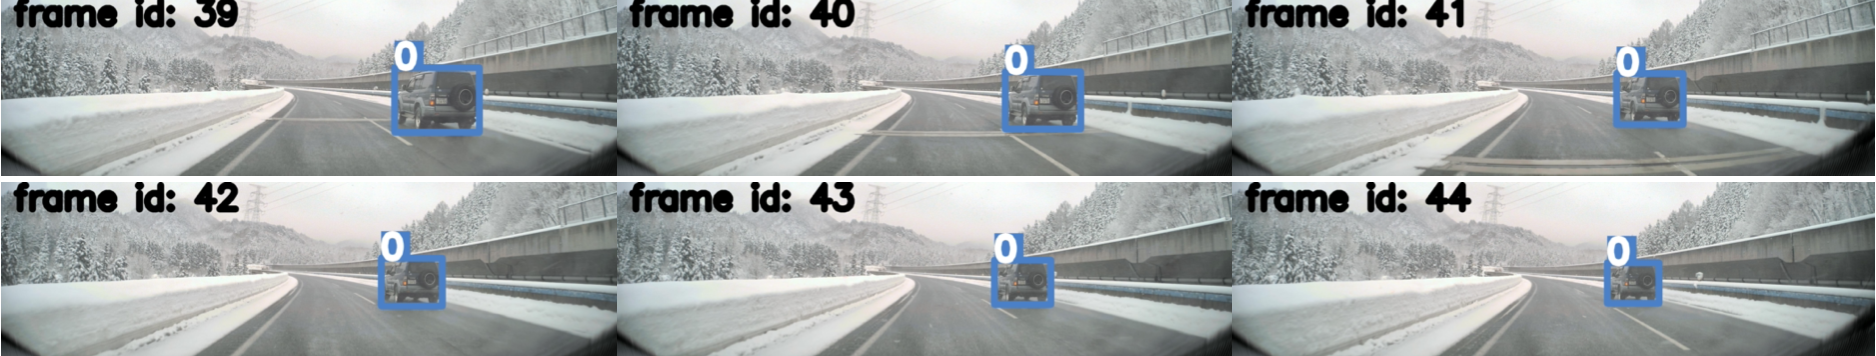
\includegraphics[width=1.05\textwidth]{pics/track01.png}
		\caption{Detect \& track objects on continuous frames.}
	\end{figure}

\end{frame}

\begin{frame}
	\frametitle{Inference Results of a Tracker}

	Finally, the inference results should \emph{locate objects},
	\emph{maintain their ids},
	and \emph{yield individual trajectories}.

	\begin{figure}
		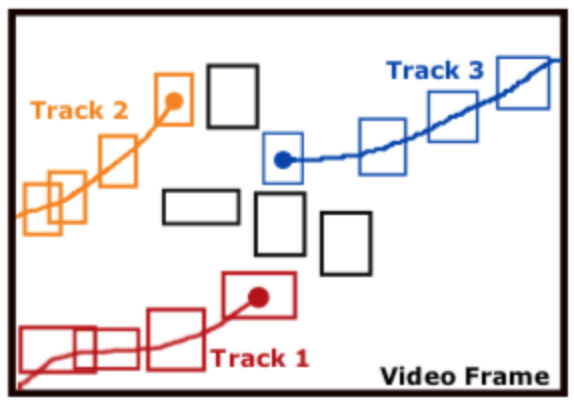
\includegraphics[height=90pt]{pics/fig1.png}
		\caption{Trajectories and several un-tracked / isolated predictions.}
	\end{figure}

\end{frame}

\begin{frame}
	\frametitle{To Evaluate a Tracker}

	To evaluate a tracker, we compare the inference results with ground-truths.

	\quad

	Similarly, the ground-truths also contain
	\begin{itemize}
	\item \emph{locations of objects} (denoted by gtObjs, gtDets) and
	\item their \emph{identities}.
	\end{itemize}
	And objects with the same id also form a trajectory.

	\quad

	A {\bf metric} here is used to measure the difference between
	ground-truths and the predictions (hypotheses).

\end{frame}

\begin{frame}
	\frametitle{To Evaluate a Tracker}

	We think a tracker is {\bf good} if
	\emph{the ids it assigns to the same objects are consistent in different frames}.
	However, this is also based on the performance of its detection part.

	\begin{figure}
		\begin{subfigure}{.48\textwidth}
		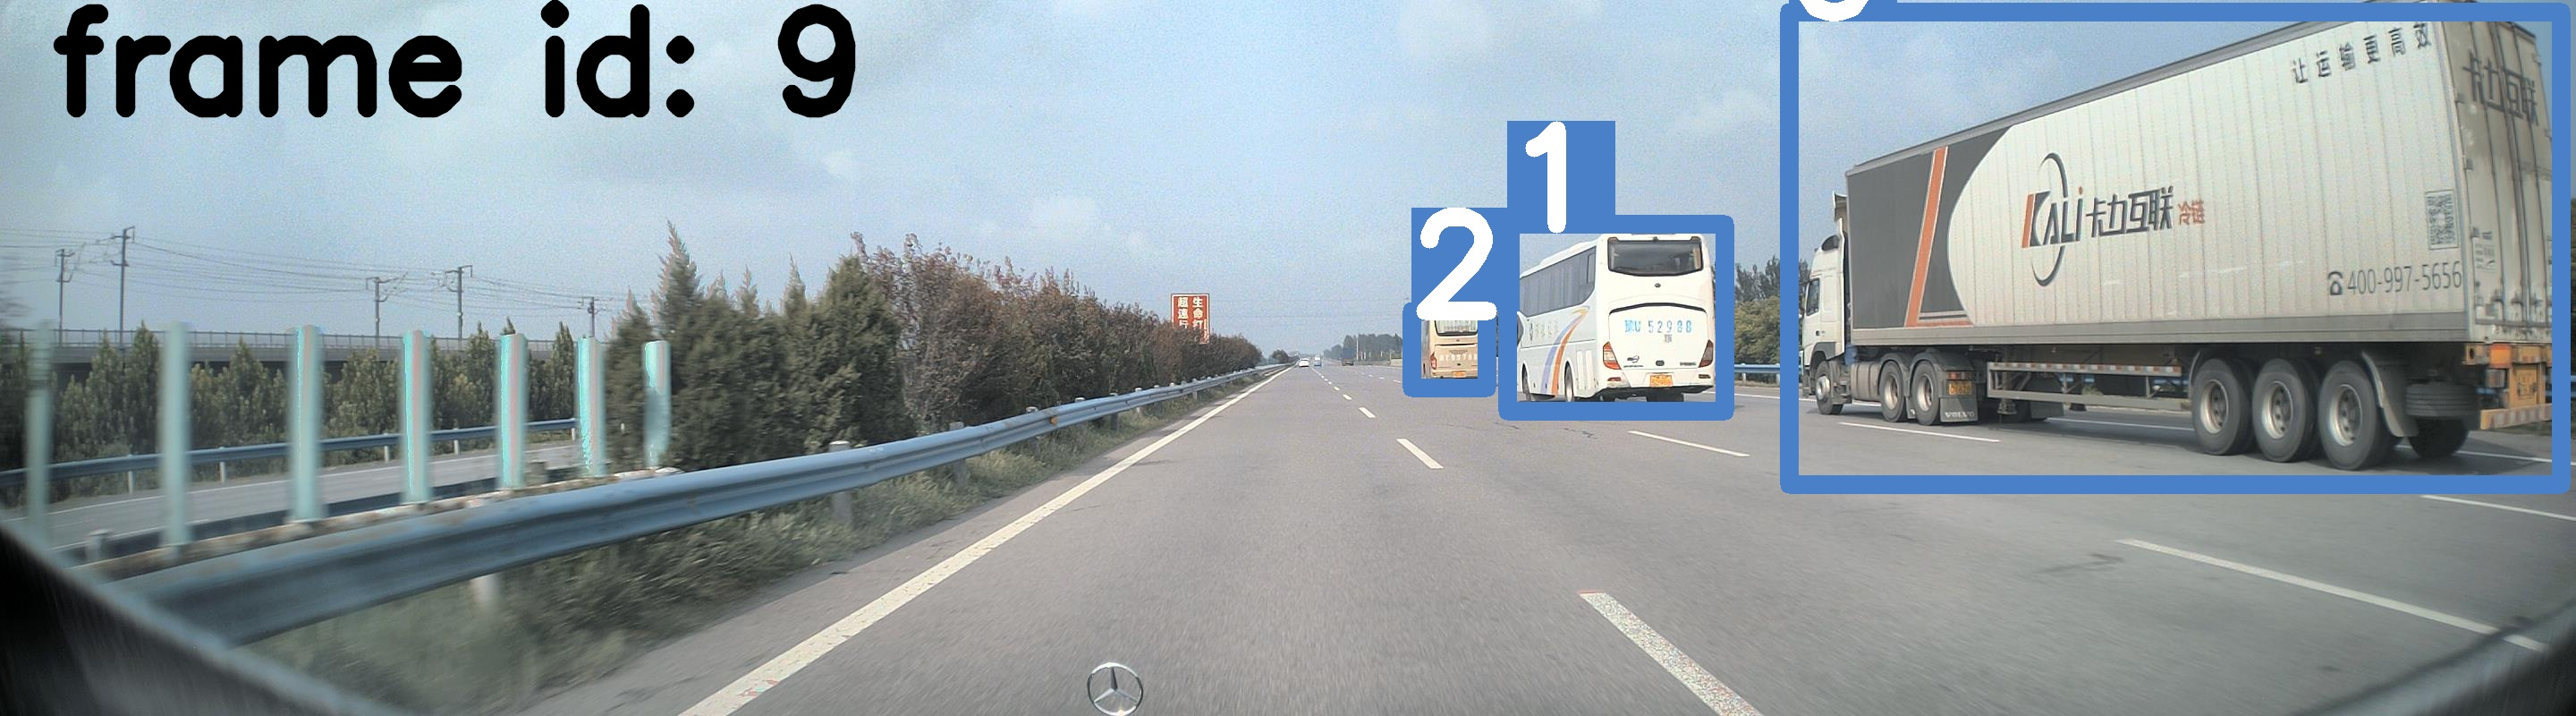
\includegraphics[width=150pt]{pics/track03.jpg}
		\end{subfigure}
		\begin{subfigure}{.48\textwidth}
		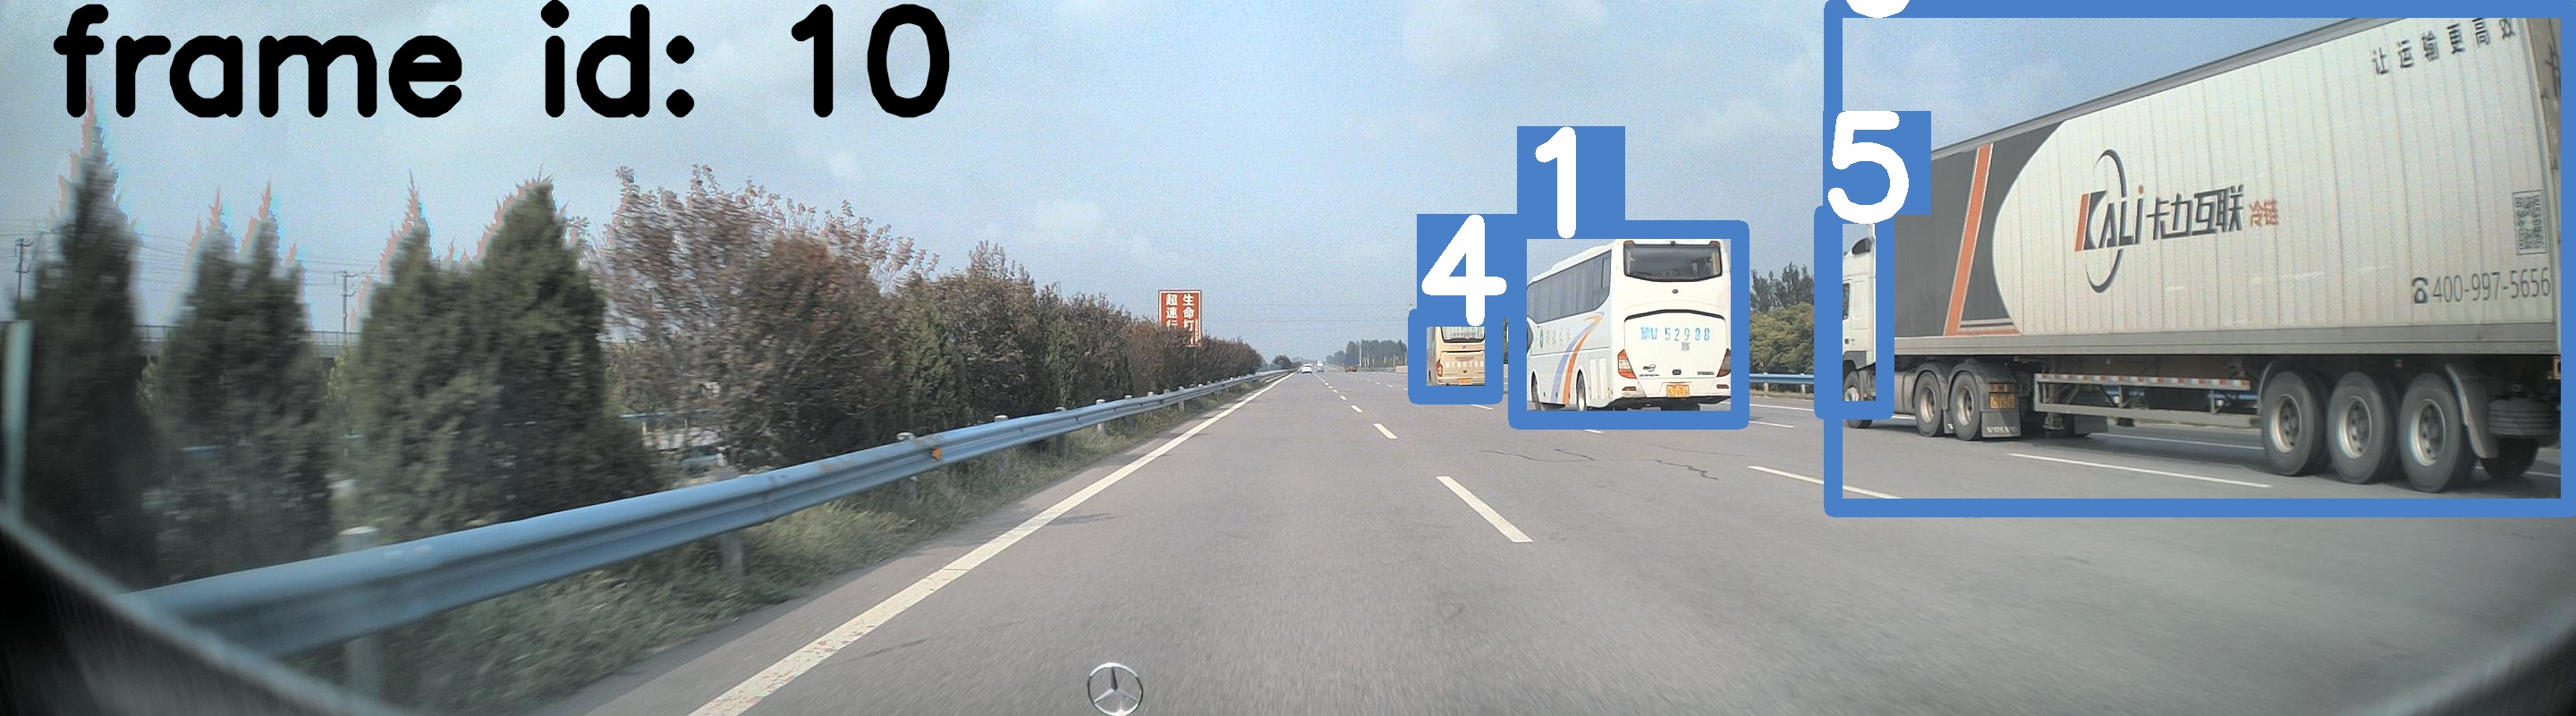
\includegraphics[width=150pt]{pics/track04.jpg}
		\end{subfigure}
		\caption{{\color{red}\bf [NG cases]} Fail to track the id 2.
			Wrong detection on the id 5.}
	\end{figure}

	To see the consistence, we firstly match detections to the ground-truths
	and see further if objects and ids are correctly tracked.

\end{frame}

\section{Matchings and Associations}

\begin{frame}
	\frametitle{Matching in Detection Levels}
			
	Matchings are done according to their {\bf similarity scores}.
	
	$\max\{1-\text{dist}, 0\}$ or IoU
	are often used as scoring functions.
			
	\begin{figure}
		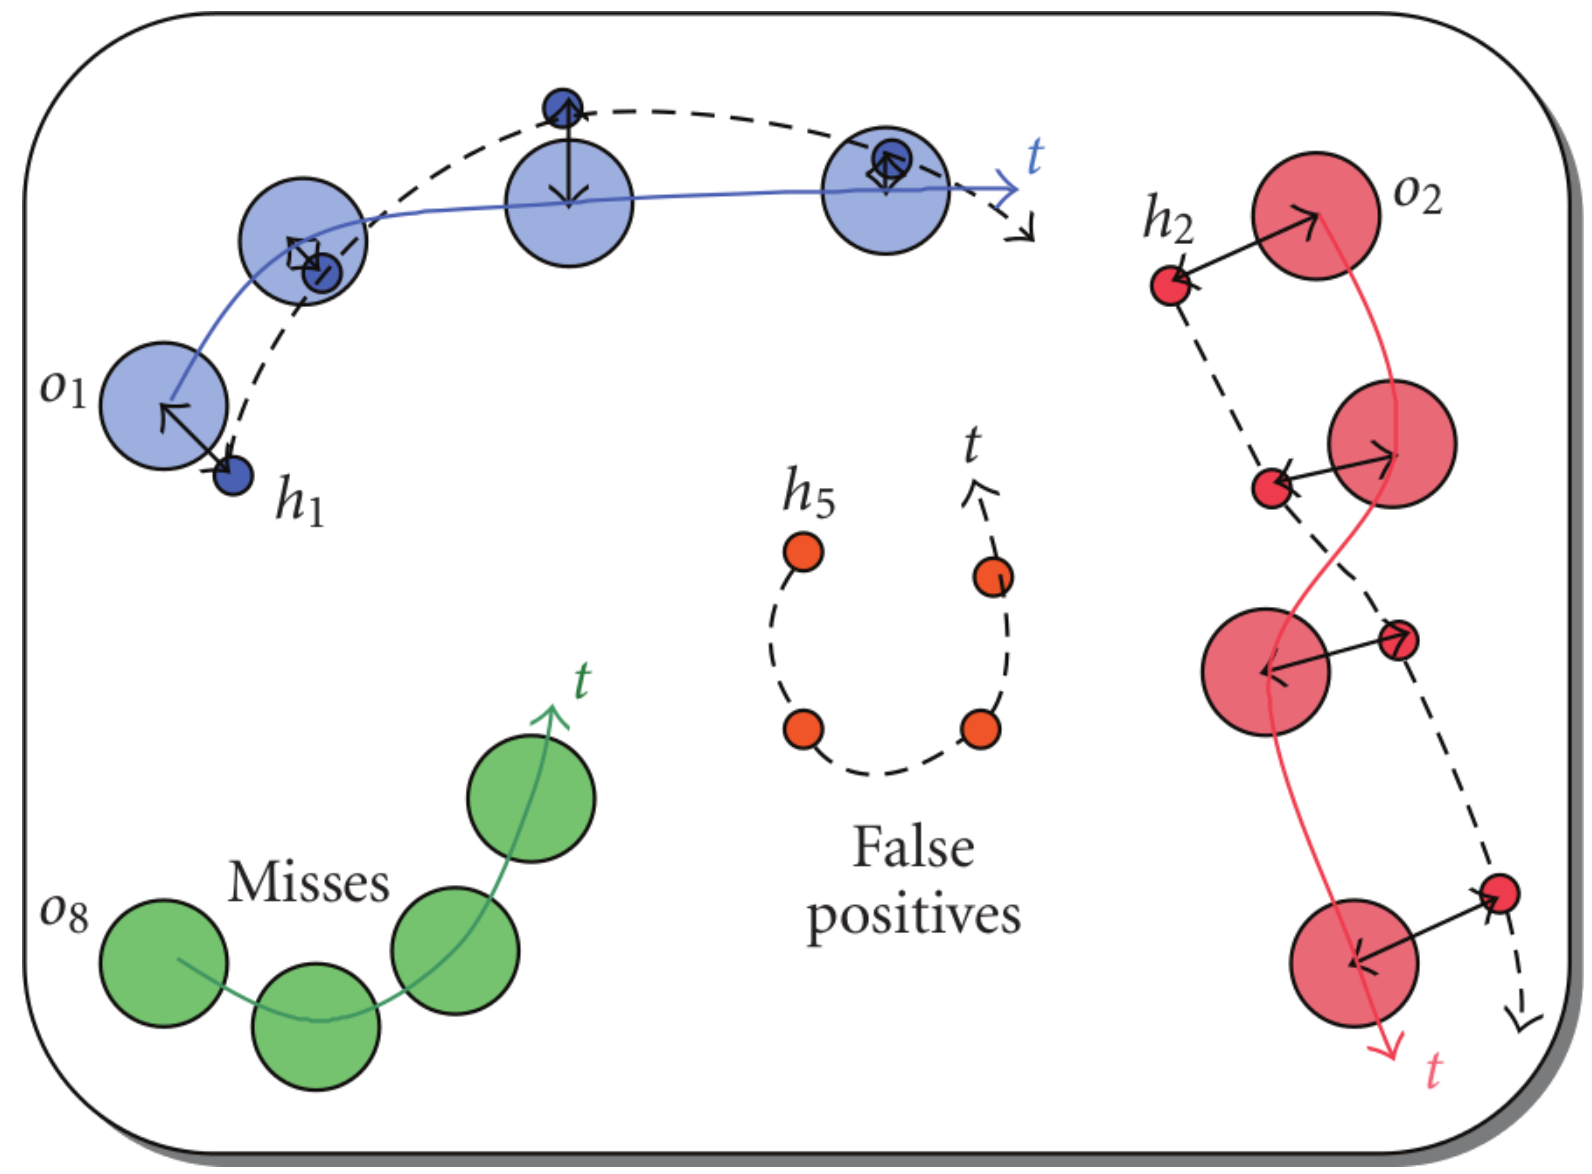
\includegraphics[width=150pt]{pics/fig2.png}
		\caption{Matchings (1-1 relation), false positives and misses in consecutive frames.
		Here the similarity is measured by the central distances.}
	\end{figure}

\end{frame}

\begin{frame}
	\frametitle{Similarity Threshold and the Performance Measures}
		
	Denote the similarity function by $\mathcal S$.
	To filter out bad matches, a threshold $\alpha$ is given.
	Once a matching $\Pi_\alpha$ under threshold $\alpha$ is done, it satisfies
	\[
		\forall\ (g,p)\in\Pi_\alpha, ~ \mathcal S(g,p) \geq \alpha.
	\]
	Hence we can define the following measures in the detection level.
	\begin{itemize}
		\item TP, TP$_\alpha$: matched pairs in a matching $\Pi_\alpha$.
		\item FP, FP$_\alpha$: non-matched predictions.
		\item FN, FN$_\alpha$: non-matched ground-truths.
	\end{itemize}
	{\color{red} Remark: For an $\alpha$, there may be several matchings fulfilling this threshold.}
\end{frame}

\begin{frame}
	\frametitle{Notations}
			
	\begin{itemize}
		\item A matching $\Pi$ can be a matching in a frame $f$ and specified by $\Pi^{(f)}$;
		      or be a matching during all frames.
		\item When $\Pi$ denotes a global matching of objects, it is the union of all its sections:
		      $\Pi = \cup_{f\in F}\Pi^{(f)}$ ($F$ collection of all frames).
		\item Furthermore, once a set $E$ is well-defined in each frame,
		      we denote $E^{(f)}$ as the $f$-section, i.e. elements in frame $f$.
		      		      		      
	\end{itemize}
			
	\vspace{-2pt}

	For a ground-truths $g$ or a prediction $p$, denote
	\begin{itemize}
		\item $f_g$ / $f_p$ as the frame it appears;
		\item $\text{gtId}(g)$ / $\text{prId}(p)$ as its id;
		\item $\text{gtTr}(g)$ / $\text{prTr}(p)$ as its trajectory.
	\end{itemize}

\end{frame}

\begin{frame}
	\frametitle{IDSW in Consecutive Frames}
			
	An {\bf IDSW (id switch)} event means there exist TP pairs, say $(g_i, p_j)\in\Pi^{(f)}$,
	$(g_k, p_\ell)\in\Pi^{(f+1)}$, in two consecutive frames
	$f$ and $f+1$ that satisfy
	\[
		\text{gtId}(g_i) = \text{gtId}(g_k),\ 
		\text{prId}(p_j) \neq \text{gtId}(p_\ell).
	\]
	Actually, this is an \emph{id mismatch} occuring in frame $f+1$.
	If two objects exchange their ids in new frame, then this is regarded as two
	IDSW events.
	\begin{figure}
		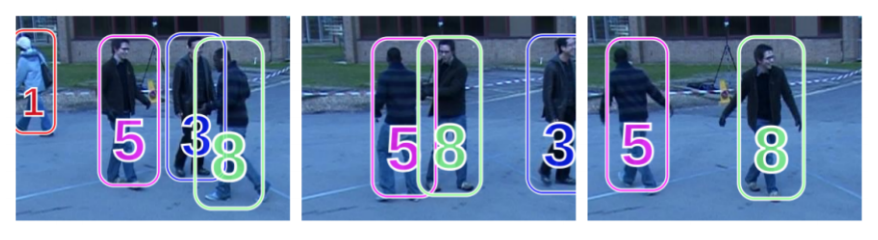
\includegraphics[width=180pt]{pics/fig3.png}
		\caption{The ids 3 \& 8 exchanges. Two IDSW events.}
	\end{figure}
			    
\end{frame}

\begin{frame}
	\frametitle{IDSWs Caused by ID-Exchange and Losing Tracks}

	\begin{figure}
		\begin{subfigure}{.49\textwidth}
			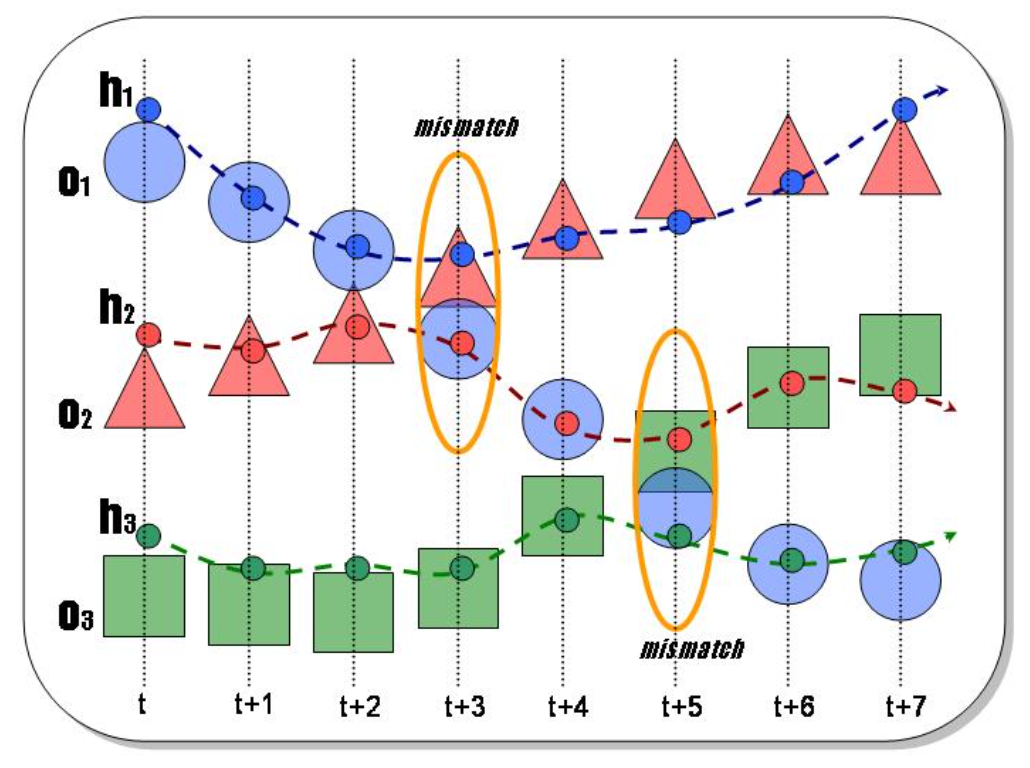
\includegraphics[width=150pt]{pics/fig16.png}
		\end{subfigure}
		\begin{subfigure}{.49\textwidth}
			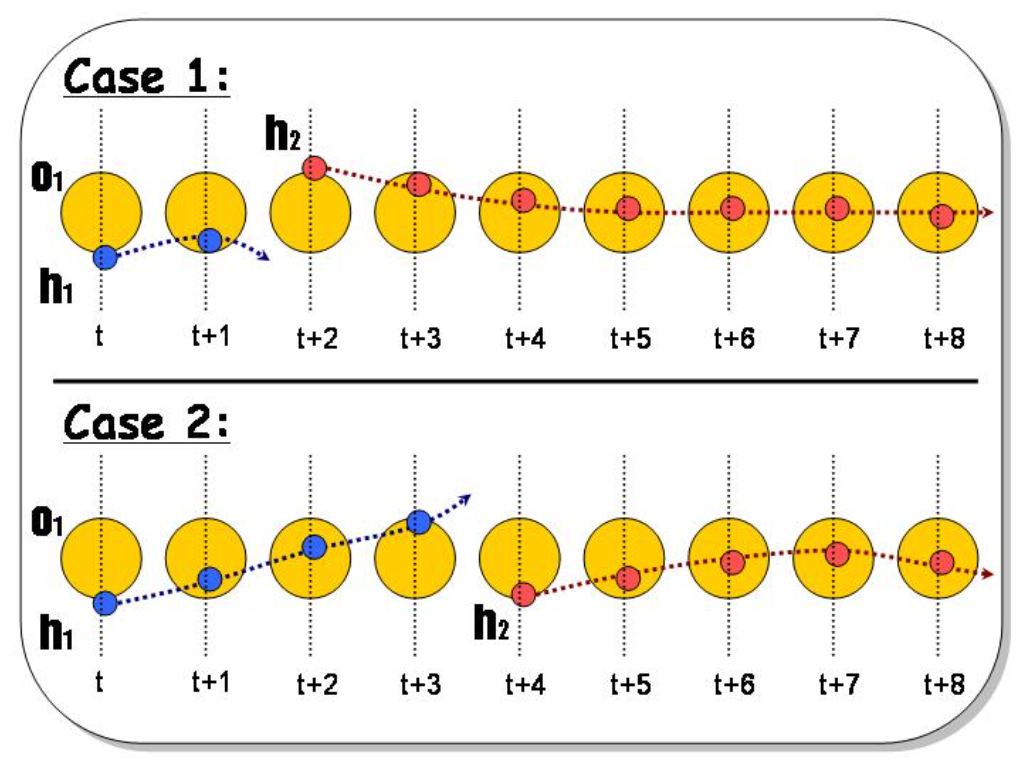
\includegraphics[width=150pt]{pics/fig17.png}
		\end{subfigure}
		\caption{Cases of losing tracks.}
	\end{figure}
\end{frame}

\begin{frame}
	\frametitle{Tracking Accuracy: A First Meet.}

	Now by utilizing measures introduced above,
	we have a simple metric to evaluate the performance.
	Instead of measuring the difference,
	we'd like to use a `score` to present how good it is.

	\vspace{3pt}

	The tracking errors consist of:
	\begin{itemize}
	\item \emph{an id switch event}, or that
	\item \emph{an object is out of detection}, or a \emph{wrong prediction}.
	\end{itemize}

	The MOTA (multiple object tracking accuracy) score is defined by
	\[
		\text{MOTA} = 1 - \dfrac{|\text{FP}| + |\text{FN}| + |\text{IDSW}|}{|\text{gtDets}|}.
	\]
	The range of MOTA is $(-\infty,1]$. As FP, FN, IDSW increase, the MOTA value decrease.

\end{frame}


\begin{frame}
	\frametitle{Discussion on MOTA}

	\begin{minipage}{50pt}
		\begin{figure}
			
\includegraphics[width=50pt]{pics/question2.png}
		\end{figure}
	\end{minipage}
	\begin{minipage}{250pt}
	\begin{itemize}
	\item Which hypothesis id is matched to ground-truth id? for most frames?
	\item When MOTA is much lower from $1$, we don't know either detectors or tracking result is worse.
	\item Sometimes IDSW can't help distinguish the exchange of two ids or
		losing and re-tracking an object with id.
	\end{itemize}
	\end{minipage}

	\vspace{10pt}

	In the following, matching in trajectory levels is investigated.

\end{frame}

% \subsection{Matching in Trajectory Levels}

\begin{frame}
	\frametitle{Matching in Trajectory Levels}

	A sketch of a matched pair of trajectories.
	\begin{figure}
		\begin{subfigure}{.5\textwidth}
			\centering
			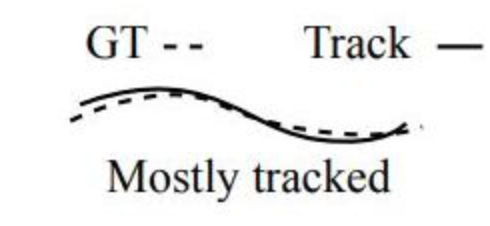
\includegraphics[width=130pt]{pics/fig4.png}
		\end{subfigure}%
		\begin{subfigure}{.5\textwidth}
			\centering
			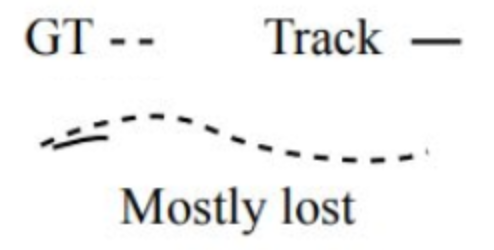
\includegraphics[width=115pt]{pics/fig5.png}
		\end{subfigure}
		\caption{Mostly tracked \& mostly lost.}
	\end{figure}

	\vspace{-5pt}

	A trajectory-to-trajectory matching $\leftrightarrow$ A gtid-to-prid matching.
	
	\quad

	To match trajectories, the similarity scores of trajectories are
	measured by the similarities of detections.
			
\end{frame}

\begin{frame}
	\frametitle{Similarity of Trajectories}
			
	Similarities are measured
	by counting overlapping and the rest parts of each pair of trajectories.
			
	\vspace{5pt}
			
	Let $\mathfrak g$, $\mathfrak p$ be a pair
	and $\alpha$ be a (detection-) similarity threhold.
	We can also define the analogues:

	\vspace{5pt}

	\begin{itemize}
		\item $\mathds{TP}$, $\mathds{TP}_{\mathfrak g, \mathfrak p}$:
		      the overlapping part of $\mathfrak g$ and $\mathfrak p$.
		      \[
		      	\mathds{TP} := \{(g,p)\ |\ 
		      	g\in\mathfrak g,~
		      	p\in\mathfrak p,~
		      	f_g=f_p,~ \mathcal S(g,p)\geq \alpha\}
		      \]
		\item $\mathds{FP}$, $\mathds{FP}_{\mathfrak g, \mathfrak p}$:
		      the non-matched predictions.
		      \begin{align*}
		      	\mathds{FP} := & \{ p\in\mathfrak p\ |\ 
		      	\nexists\ g\in\mathfrak g ~\suchthat~ \mathcal S(g,p)\geq\alpha,~ f_g=f_p.\}
		      \end{align*}
	\end{itemize}
			
\end{frame}

\begin{frame}
	\frametitle{Similarity of Trajectories}
			
	\begin{itemize}
		\item $\mathds{FN}$, $\mathds{FN}_{\mathfrak g, \mathfrak p}$: the non-matched ground-truth objects.
		      \begin{align*}
		      	\mathds{FN} := & \{ g\in\mathfrak g\ |\ 
		      	\nexists\ p\in\mathfrak p ~\suchthat~ \mathcal S(g,p)\geq\alpha,~ f_p=f_g.\}
		      \end{align*}
	\end{itemize}
			
	The similarity of trajectories is defined by
	\[
		\mathcal S_{\rm tr}(\mathfrak g, \mathfrak p) :=
		\dfrac{|\mathds{TP}_{\mathfrak g,\mathfrak p}|}{
			|\mathds{TP}_{\mathfrak g,\mathfrak p}|+|\mathds{FP}_{\mathfrak g,\mathfrak p}|+|\mathds{FN}_{\mathfrak g,\mathfrak p}|
		}
	\]
	Once the similarities are calculated,
	the matching of trajectories can be done by Hungarian algorithms.
\end{frame}


\begin{frame}
	\frametitle{Performance Measures Focusing on IDs}
			
	Suppose a matching of trajectories are done and denoted by $\mathfrak P$,
	we can define the performance measures as follows.
			
	\vspace{4pt}
			
	Again, denote $\alpha$ as the (detection-) similarity threshold.
	\begin{itemize}
		\item IDTP:
		      the overlapping part of all $(\mathfrak g, \mathfrak p) \in \mathfrak P$.
	\end{itemize}
			
	\vspace{-15pt}
	\[
		\text{IDTP} := \left\{ (g,p)\ |\ 
		g\in\mathfrak g, ~ p\in\mathfrak p, ~
		f_g=f_p, ~ 
		\mathcal S(g,p) \geq \alpha, ~ 
		(\mathfrak g, \mathfrak p)\in\mathfrak P
		\right\}
	\]
	\vspace{-10pt}
	\begin{itemize}
		\item IDFP:
		      non-matched predictions in matched pairs
		      and all predictions in non-matched predictive trajectories.
	\end{itemize}
	\begin{align*}
	\text{IDFP} := & \left\{ p\in\text{prDets}\ \left|\                                                
	\mathcal S(g,p)<\alpha, \ 
	\forall\ g\in\mathfrak g^{(f_p)},
	(\mathfrak g,\mathfrak p)\in\mathfrak P.
	\right.
	\right\} \\
					& \bigcup \left\{p \in \text{prDets}\ |\ \text{prTraj$(p)$ is not matched.}\right\} 
	\end{align*}
			    
\end{frame}

\begin{frame}
	\frametitle{Performance Measures Focusing on IDs}
	\begin{itemize}
		\item IDFN:
		      non-matched ground-truths in matched pairs and
		      all ground-truths in non-matched ground-truth trajectories.
	\end{itemize}

	\vspace{-15pt}
	\begin{align*}
		\text{IDFN} := & \left\{ g\in\text{gtDets}\ \left|\                                                
		\mathcal S(g,p)<\alpha, \ 
		\forall\ p\in\mathfrak p^{(f_g)},
		(\mathfrak g,\mathfrak p)\in\mathfrak P
		\right.
		\right\} \\
		               & \bigcup \left\{g \in \text{gtDets}\ |\ \text{gtTraj$(g)$ is not matched}\right\}. 
	\end{align*}
	
	By these quantities, the id-matchings can be evaluated by
	\[
		\text{ID-Precision} := \dfrac{|\text{IDTP}|}{|\text{IDTP}| + |\text{IDFP}|},
		\quad
		\text{ID-Recall} := \dfrac{|\text{IDTP}|}{|\text{IDTP}| + |\text{IDFN}|},
	\]

	\vspace{-10pt}
	\[
		\text{IDF1} := \dfrac{|\text{IDTP}|}{|\text{IDTP}| + 0.5|\text{IDFP}| + 0.5|\text{IDFN}|}.
	\]
\end{frame}

\begin{frame}
	\frametitle{Discussion on the ID-Metrics}
			
	By observations, the id-metrics show how good the trackings are.

	\quad

	But once if several fragmentations occur in different frames,
	then we cannot not distinguish this case with the mostly lost cases.

	\vspace{5pt}
			
	\begin{figure}
		\begin{subfigure}{.5\textwidth}
			\centering
			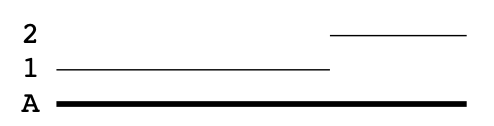
\includegraphics[width=120pt]{pics/fig6.png}
		\end{subfigure}%
		\begin{subfigure}{.5\textwidth}
			\centering
			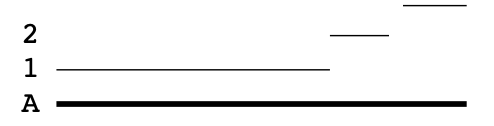
\includegraphics[width=120pt]{pics/fig7.png}
		\end{subfigure}
		\caption{The id metrics only measure tracking results of matched peices.
		The ground-truth id is shown by the bold line.}
	\end{figure}
			
\end{frame}

\begin{frame}
	\frametitle{Problems in Matching Trajectories}
			
	\begin{itemize}
		\item {\bf fragmentations}:
		      A ground-turth trajectory is matched by
		      several predictive trajectories.
		\item {\bf merge}:
		      A hypothetical trajectory is matched to several ground-truths.
	\end{itemize}
	
	\vspace{-15pt}
	\begin{figure}
		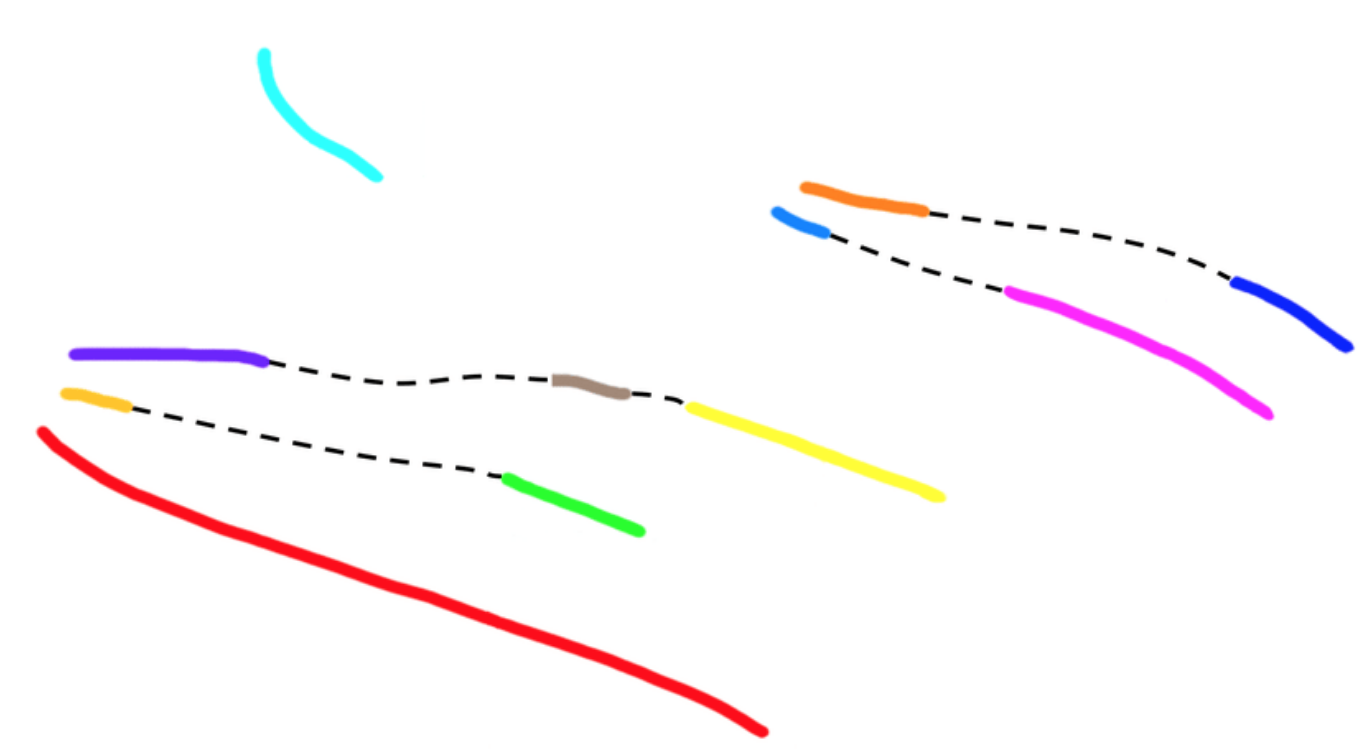
\includegraphics[width=140pt]{pics/fig9.png}
		\caption{Six objects. Colored segm's are diff. ids and dash lines are misses.}
	\end{figure}
		
	\vspace{-15pt}
	It's a drawback that trajectory matching only allows 1-1 relation.
			
\end{frame}

\begin{frame}
	\frametitle{Measures for Associations of Objects}
			
	By concepts in id-matchings,
	{\bf tracking associations of a single object} is developed in further.
	\emph{Do matching in detection levels and associate multiple ids by matching.}
			
	\vspace{5pt}
			
	Given a framewise matching $\Pi_\alpha$.
	Let $c = (g,p)$ be a TP pair in a frame $t$.
	We define TPA, FPA and FNA as follows.
	\begin{align*}
		\text{TPA}(c) :=                       
		\left\{(g_i, p_j)\in\text{TP}\ \left|\ 
		\begin{array}{c}                       
		\text{grId}(g_i)=\text{grId}(g),       \\
		\text{prId}(p_j) = \text{prId}(p)      
		\end{array}\right.                     
		\right\}.                              
	\end{align*}
	Note that $|\text{TPA}(c)|$ is also the number of frames that $\text{gtTraj}(g)$
	and $\text{prTraj}(p)$ overlap.
			
\end{frame}

\begin{frame}
	\frametitle{Measures for Associations of Objects}
			
	% Similarly, for the TP pair $c = (g, p)$, we also define the false positive associations
	% and false negative associations as follows.
	\vspace{-20pt}
	\begin{align*}
		\text{FPA}(c) := &             
		\left\{(g_i, p_j)\in\text{TP}\ \left|\ 
		\begin{array}{c}
		\text{grId}(g_i) \neq \text{grId}(g), \\
		\text{prId}(p_j) = \text{prId}(p)
		\end{array}\right.
		\right\} \\
		                 & ~ \bigcup ~ 
		\Big\{p_j\in\text{FP}\ |\ 
		\text{prId}(p_j) = \text{prId}(p)
		\Big\}; \\
		\text{FNA}(c) := &             
		\left\{(g_i, p_j)\in\text{TP}\ \left|\ 
		\begin{array}{c}
		\text{grId}(g_i) = \text{grId}(g), \\
		\text{prId}(p_j) \neq \text{prId}(p)
		\end{array}\right.
		\right\} \\
		                 & ~ \bigcup ~ 
		\Big\{g_i\in\text{FN}\ |\ 
		\text{gtId}(g_i) = \text{gtId}(g)
		\Big\}.
	\end{align*}
	Note that $\text{FPA}(c)$ and $\text{FNA}(c)$ relate to the non-matched
	or id-mismatched objects in $\text{prTraj}(p)$ and $\text{grTraj}(g)$.
			
\end{frame}

\begin{frame}
	\frametitle{Tracking Accuracy of a Single Matched Pair}

	Under a framewise matching, for a TP pair $c=(g,p)$,
	the tracking accuracy of the id-matching $(\text{grId}(g), \text{prId}(p))$
	is
	\[
		\mathcal A(c) := 
		\dfrac{|\text{TPA}(c)|}{|\text{TPA}(c)|+|\text{FPA}(c)|+|\text{FNA}(c)|}.
	\]
	This value shows how good the association $(\text{grId}(g), \text{prId}(p))$ is.
	And we can compare these accuracies calculated from different pairs
	of id-matchings.

	\vspace{5pt}

	Better than the id-metrics, the tracking accuracy $\mathcal A$ gives
	\emph{partial credits} on small peices of matched trajectories.

\end{frame}

\begin{frame}
	\frametitle{An Example of Tracking Associations}
	\begin{figure}
		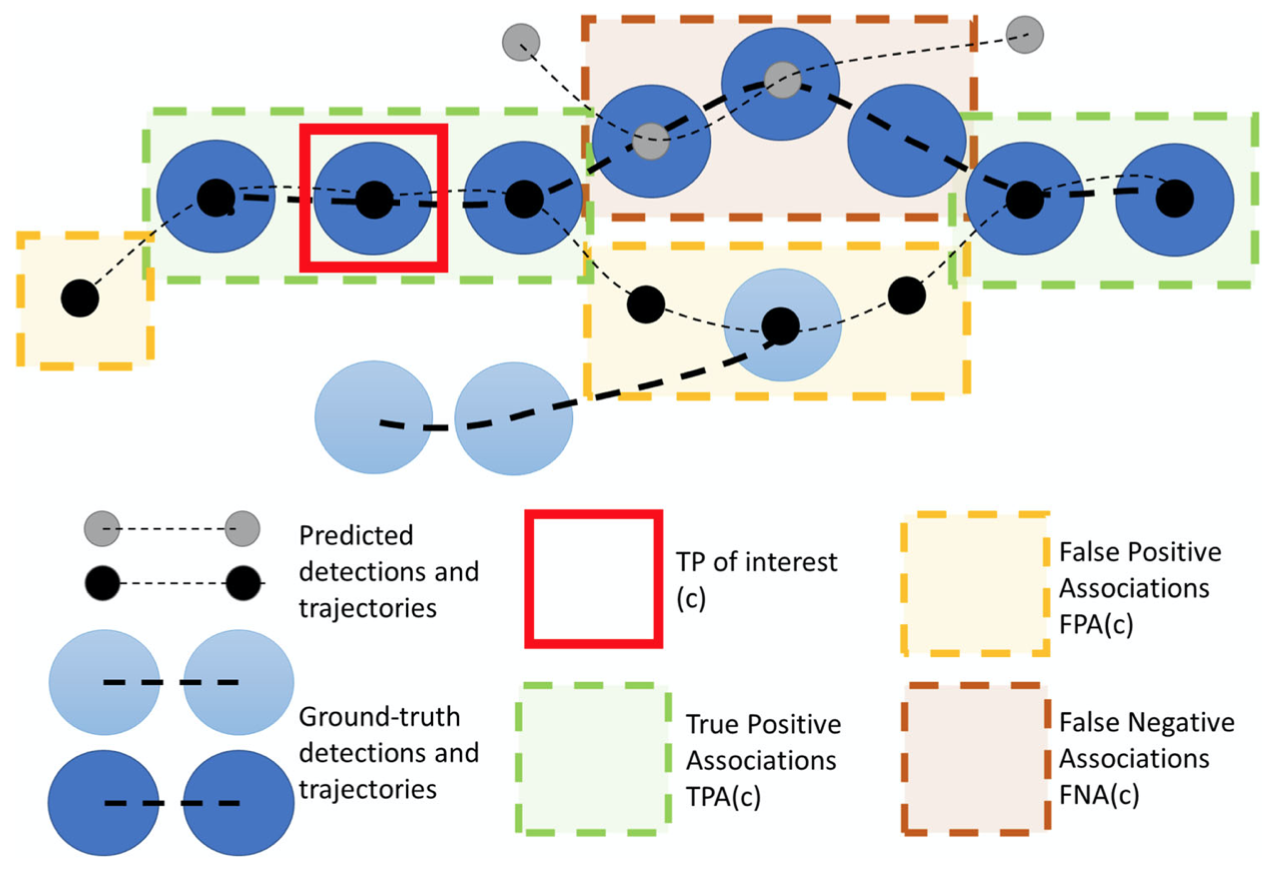
\includegraphics[width=240pt]{pics/fig8.png}
		\caption{For the interested object (red box), TPA: 5; FPA: 4; FNA: 3.}
	\end{figure}
\end{frame}

\section{The Metrics}

\begin{frame}
	\frametitle{Metrics for Evaluating Trackers}
			
	Again, we recall that \emph{performance of object trackings is based 
	on the result of detections}.
			
	\vspace{5pt}

	In more details than before,
	metrics often consists of the following aspects
	\begin{itemize}
		\item detection;%: measure accuracies of predictions
		\item localization;%: measure accuracies of positions of correct predictions
		\item association.%: measure accuracies of the correct associations of objects
	\end{itemize}

	In the following, we'll restate the definitions of the common used metrics
	mentioned above carefully and introduce the HOTA metrics.

\end{frame}

% \subsection{CLEAR-MOT: MOTA and MOTP}

\begin{frame}
	\frametitle{CLEAR-MOT: MOTA and MOTP scores}
			
	% {\scriptsize\tt K. Bernardin \& R. Stiefelhagen, Evaluating Multiple Object Tracking Performance:%
	% The CLEAR MOT Metrics.}
			
	Given a similarity threshold $\alpha\in (0,1)$.
			
	\vspace{4pt}
			
	{\bf MOTA (multiple object tracking accuracy)} is calculated through
	\emph{optimizing the value}
	\[
		\text{MOTA}_\alpha :=
		\max_{\Pi_\alpha}
		\left\{1 - \dfrac{|\text{FN}_{\Pi_\alpha}| + |\text{FP}_{\Pi_\alpha}| + |\text{IDSW}_{\Pi_\alpha}|}{|\text{gtDet}|}\right\}
	\]
	among all matchings $\Pi_\alpha$ with $\mathcal S(c)\geq \alpha$ for all matched $c\in\Pi_\alpha$.
			
	\vspace{4pt}
			
	{\bf\color{blue} The FN, FP term may stand for the accuracy of detections.} \\
	{\bf\color{olive} The IDSW term may stands for the accuracy of associations.}
			
	\vspace{4pt}
		
	Remark: under $\alpha$, the matching is taken to optimize $|\text{TP}|$ as well.
			
\end{frame}

\begin{frame}
	\frametitle{CLEAR-MOT: MOTA and MOTP scores}
			
	As the MOTA score is achieved by some matching $\Pi_\alpha$, {\bf MOTP (multiple object tracking precision)}
	is calculated as follows:
	\[
		\text{MOTP}_\alpha =
		\dfrac{\sum_{(g,p)\in\text{TP}_{\Pi_\alpha}}\mathcal S(g,p)}{|\text{TP}_{\Pi_\alpha}|}.
	\]
	{\bf\color{red} MOTP measures the accuracy of localizations of predictions}.
			
	\vspace{4pt}
			
	As mentioned before, if the MOTA value is low,
	then somehow it cannot be distinguished that
	the detections are not good or the tracking results are not good.
			
	\vspace{5pt}
		
	$\alpha\nearrow$ $\Rightarrow$ $|\text{FN}|, |\text{FP}|, \mathcal S \nearrow$, $|\text{TP}| \searrow$ $\Rightarrow$ MOTP $\nearrow$.
	$|\text{IDSW}|, \text{MOTA}$ $?$
	
\end{frame}

\begin{frame}
	\frametitle{The ID Metrics}
			

	The id metrics focus on matching of trajectories.
			
	\vspace{5pt}
			
	Under a similarity threshold $\alpha$, the scoring functions are calculated
	through optimizing the quantity $|\text{IDTP}|$ among matchings $\mathfrak P$
	in trajectory level as follows:
	\begin{align*}
		\text{ID-Precision} := & ~ \max_{\mathfrak P} \dfrac{|\text{IDTP}|}{|\text{IDTP}| + |\text{IDFP}|}, \\
		\text{ID-Recall} :=    & ~ \max_{\mathfrak P}\dfrac{|\text{IDTP}|}{|\text{IDTP}| + |\text{IDFN}|},  \\
		\text{IDF1} :=         &                                                                            
		~ \max_{\mathfrak P}\dfrac{|\text{IDTP}|}{|\text{IDTP}| + 0.5|\text{IDFP}| + 0.5|\text{IDFN}|}.
	\end{align*}

	$\alpha\nearrow$ $\Rightarrow$ $|\text{IDTP}|\searrow$,
	$|\text{IDFP}|$, $|\text{IDFN}|$ ID-Precision, ID-Recall, ID-F1 $?$

\end{frame}

\begin{frame}
	\frametitle{The HOTA metrics}
		
	The {\bf HOTA (higher order tracking accuracy)} score for a threshold $\alpha$ is defined by
	optimizing the following value among matchings in the detection level:
	\[
		\text{HOTA}_\alpha := 
		\max_{\Pi_\alpha} \sqrt{\dfrac{\sum_{c\in\text{TP}} \mathcal A(c) }{|\text{TP}|+|\text{FN}|+|\text{FP}|}},
	\]
	where $\mathcal A(c)$ is defined by
	\[
		\mathcal A(c) = \dfrac{|\text{TPA}(c)|}{|\text{TPA}(c)|+|\text{FPA}(c)|+|\text{FNA}(c)|}.
	\]
	Note that all measures TP, FP, FN, TPA, FPA, FNA depend on matching $\Pi_\alpha$.
		
\end{frame}

\begin{frame}
	\frametitle{The HOTA metrics}
	The HOTA score is defined in a double Jaccard indices way.
	It can be divided into multiples of two values:
	Once the matching $\Pi$ is defined,
	\[
		\text{AssA}_\alpha = \dfrac{1}{|\text{TP}|} \sum_{c\in\text{TP}} \mathcal A(c), \ \ 
		\text{Det}_\alpha = \dfrac{|\text{TP}|}{|\text{TP}| + |\text{FP}| + |\text{FN}|}.
	\]
	Then we have the formula:
	\[
		\text{HOTA}_\alpha = \sqrt{\text{AssA}_\alpha \cdot \text{Det}_\alpha}.
	\]
	The two scores indicate the \emph{accuracy of tracking associations}
	and the \emph{accuracy of detections}.
\end{frame}

\begin{frame}
	\frametitle{The HOTA metrics}
		
	Similarly to MOTP, by the same matching $\Pi_\alpha$,
	the localization score in HOTA is defined by
	\[
		\text{Loc}_\alpha = \dfrac{\sum_{c\in\text{TP}} \mathcal S(c)}{|\text{TP}|}.
	\]
	As a remark, $\text{AssA}_\alpha$ and $\text{Loc}_\alpha$ are not well-defined
	if $\text{TP} = \emptyset$.

	\vspace{4pt}

	Furthermore, the numerator can be changed to another metric for evaluating localizations
	(i.e. IoU, $\max\{1-\text{dist},0\}$, \ldots).
		
\end{frame}

% \section{Implementation of HOTA metrics}

% \subsection{Obtain the Optimization Matching}

% \begin{frame}
% 	\frametitle{Matching to Optimize HOTA scores}
	
% 	The optimization is done by a Hungarian algorithm for
% 	\begin{itemize}
% 		\item maximizing the number of TP pairs as the first priority;
% 		\item and maximizing the mean of association scores
% 		      as a second objective across the set of maximized TP pairs.
% 	\end{itemize}
	
% 	To reduce time cost, this is fulfilled by the following scoring MS (match score) for
% 	potential matches between each ground-truth object and prediction:
% 	\[
% 		\text{MS}(i,j) =
% 		\begin{cases}
% 			1/\epsilon + \mathcal A_{\rm max}(i,j) + \epsilon\mathcal S(i,j), & \mathcal S(i,j) \geq \alpha; \\
% 			0,                                                                & \text{otherwise}.            
% 		\end{cases}
% 	\]
	
% 	\vspace{-5pt}
% 	$\mathcal A_{\rm max}$ is a `proxy' for $\mathcal A$ (association score).
	
% \end{frame}

% \begin{frame}
% 	\frametitle{Matching to Optimize HOTA scores}
	
% 	Since the values TPA's, FNA's and FPA's of a TP pair depend on matching in other frames,
% 	\emph{the optimizing matching can not be achieved by a linear assignment formulation}.
	
% 	\vspace{5pt}
	
% 	This value is a reference for the optimizing matching and is calculated as follows.
% 	\[
% 		\mathcal A_{\rm max}(c) = 
% 		\dfrac{|\text{TPA}_{\rm max}(c)|}{|\text{TPA}_{\rm max}(c)|+|\text{FNA}_{\rm min}(c)|+|\text{FPA}_{\rm min}(c)|}.
% 	\]
% 	Here the subscriptions mean to choose the possible maximum and minimum.
% 	But in the codes provided by author of the HOTA metrics, 
% 	they are just fractions like expectation values of matches.
	
% \end{frame}

% \subsection{The Algorithm Provided by the Author of HOTA metrics}

% \begin{frame}
% 	\frametitle{The Official Calculation}
% 	\begin{figure}
% 		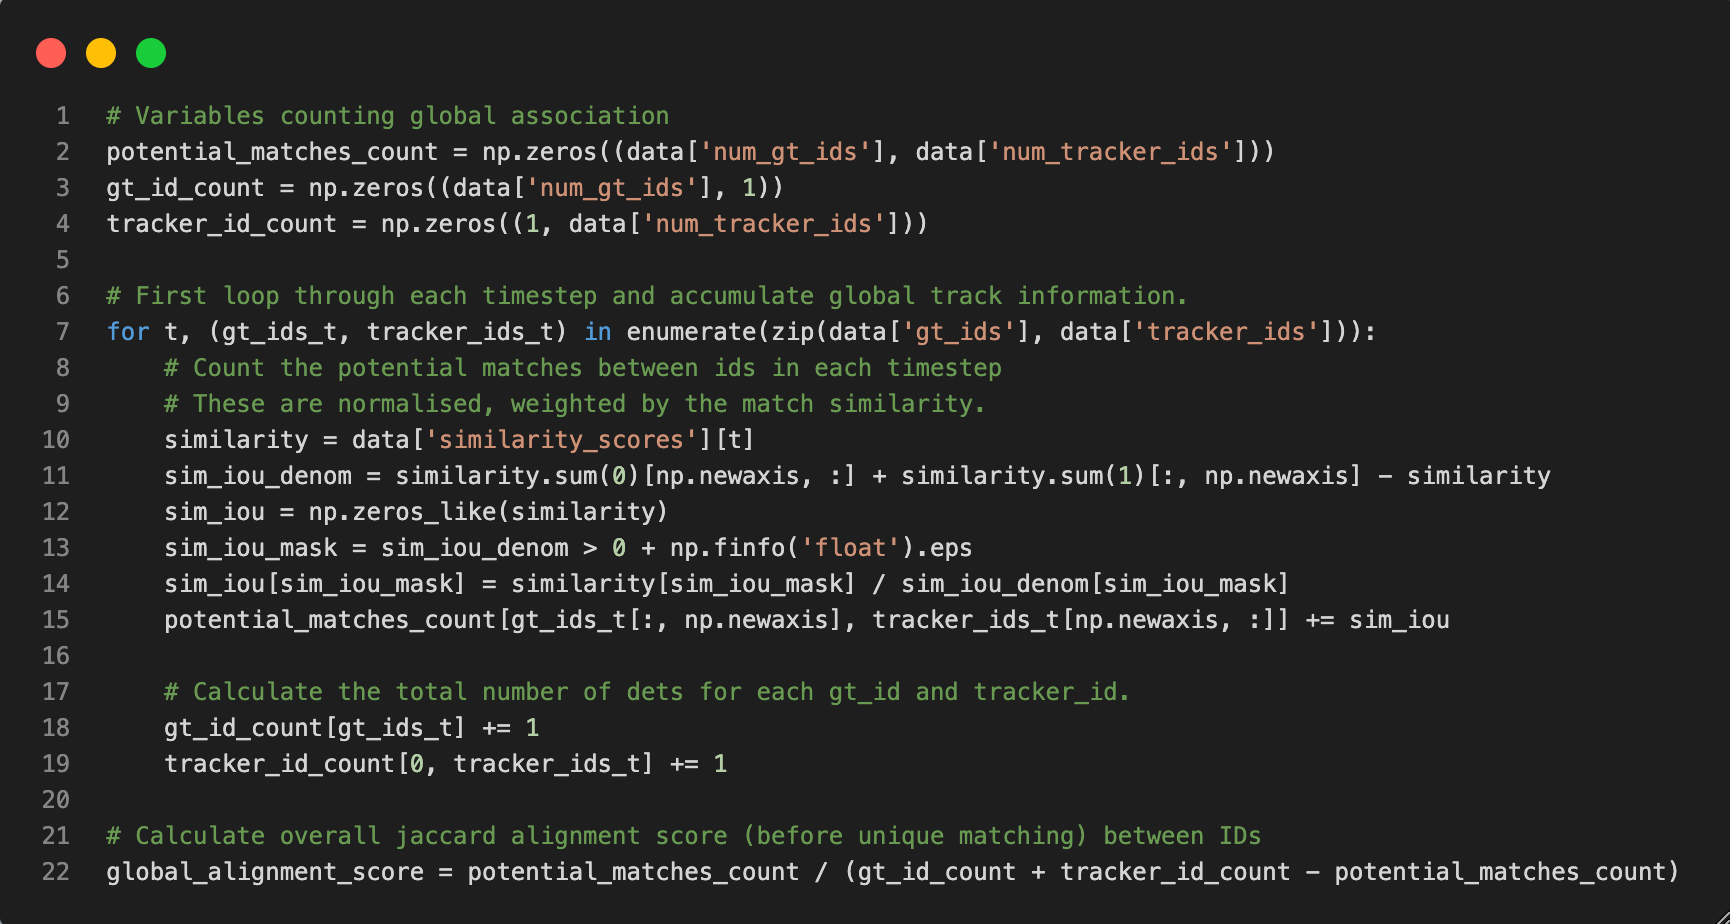
\includegraphics[width=280pt]{pics/fig10.png}
% 		\caption{Calculation of the proxies of association scores.}
% 	\end{figure}
% \end{frame}

% \begin{frame}
% 	\frametitle{The Official Calculation}
% 	\begin{itemize}
% 		\item IoU of similarities?
% 		      \begin{align*}
% 		      	\begin{bmatrix}	
% 		      	0.8                       & 0                       & 0.1                     \\
% 		      	0.5                       & 0.3                     & 0                       
% 		      	\end{bmatrix}
% 		      	\ \stackrel{\text{IoU}}{\Rightarrow}\ 
% 		      	\begin{bmatrix}
% 		      	\frac{0.8}{0.8+0+0.1+0.5} & 0                       & \frac{0.1}{0.8+0+0.1+0} \\
% 		      	\frac{0.5}{0.8+0.5+0.3+0} & \frac{0.3}{0+0.5+0.3+0} & 0                       
% 		      	\end{bmatrix} \\
% 		      	\text{(possible matches count $\approx$ TPA)}~ \Rightarrow ~ 
% 		      	\begin{bmatrix}
% 		      	4/7                       & 0                       & 1/9                     \\
% 		      	5/16                      & 3/8                     & 0                       
% 		      	\end{bmatrix}
% 		      \end{align*}
% 		\item Add this into {\scriptsize\tt `potential\_matches\_count'} according to indices.
% 		\item {\scriptsize\tt `gt\_id\_count'} and {\scriptsize\tt `track\_id\_count'} count
% 		      the numbers of frames that the ids appear. Their sum equals to $\text{FPA}+\text{FNA}+2\text{TPA}$.
% 		\item {\scriptsize\tt `global\_alignment\_score'}: the proxy value, approximation of $\mathcal A$.
		      		
% 	\end{itemize}
% \end{frame}

% \begin{frame}
% 	\frametitle{The Official Calculation}
% 	\begin{figure}
% 		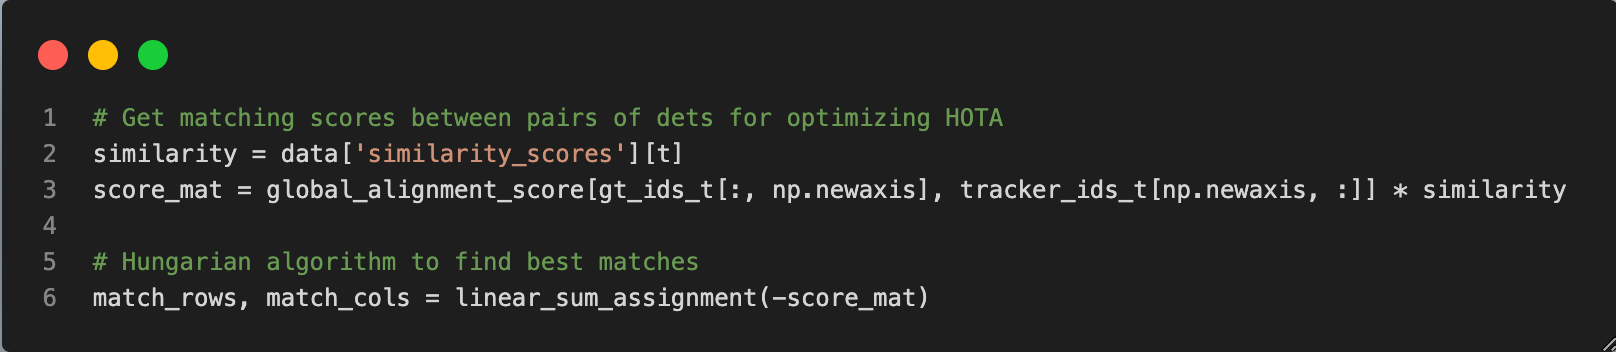
\includegraphics[width=280pt]{pics/fig11.png}
% 		\caption{Perform matching by optimizing the proxy score weighted
% 			by the local similarity via a Hungarian algorithm.}
% 	\end{figure}

% 	\vspace{-15pt}

% 	Then calculate the association scores by the `actual matching'.

% 	\vspace{3pt}

% 	By given similarity threshold $\alpha$,
% 	\begin{itemize}
% 	\item filter out matched pairs whose similarities less than $\alpha$;
% 	\item calculate the $\text{HOTA}_\alpha$ score; and
% 	\item calculate the $\text{LocA}_\alpha$ score.
% 	\end{itemize}

% \end{frame}

% \begin{frame}
% 	\frametitle{The Official Calculation: the Integration of HOTA scores}

% 	Besides of the localization score $\text{LocA}_\alpha$,
% 	integration of $\text{HOTA}_\alpha$ scores in different $\alpha$'s
% 	could also measure the performance of localization.
% 	This integration can be approximated by evaluating $\text{HOTA}_\alpha$
% 	for $\alpha$'s that partitions $[0,1]$.
% 	That is,
% 	\[
% 		\int_0^1 \text{HOTA}_\alpha~ d\alpha ~ \approx ~ \dfrac{1}{19}\sum_{\alpha\in A} \text{HOTA}_\alpha
% 	\]
% 	where $A:=\{0.05, 0.1, 0.15, \cdots, 0.9, 0.95\}$.

% \end{frame}

% \subsection{Implementation in linker-metrics}

% \begin{frame}
% 	\frametitle{Recall the Road Map of linker-metrics}

% 	\begin{figure}
% 		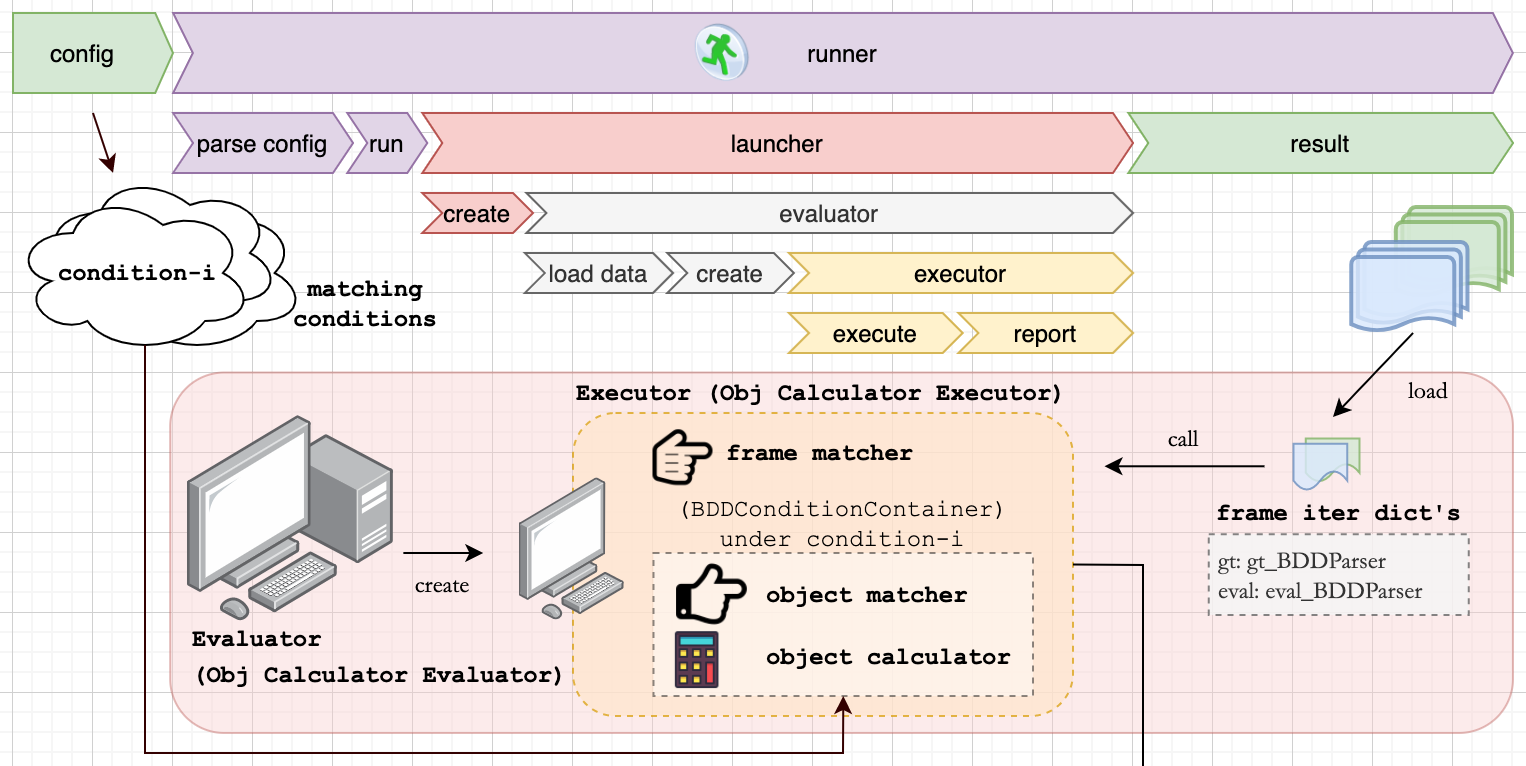
\includegraphics[width=300pt]{pics/fig12.png}
% 		\caption{runner $\to$ launcher $\to$ evaluator (calculation executor).}
% 	\end{figure}
% \end{frame}

% \begin{frame}
% 	\frametitle{Processing in linker-metrics}

% 	\begin{figure}
% 		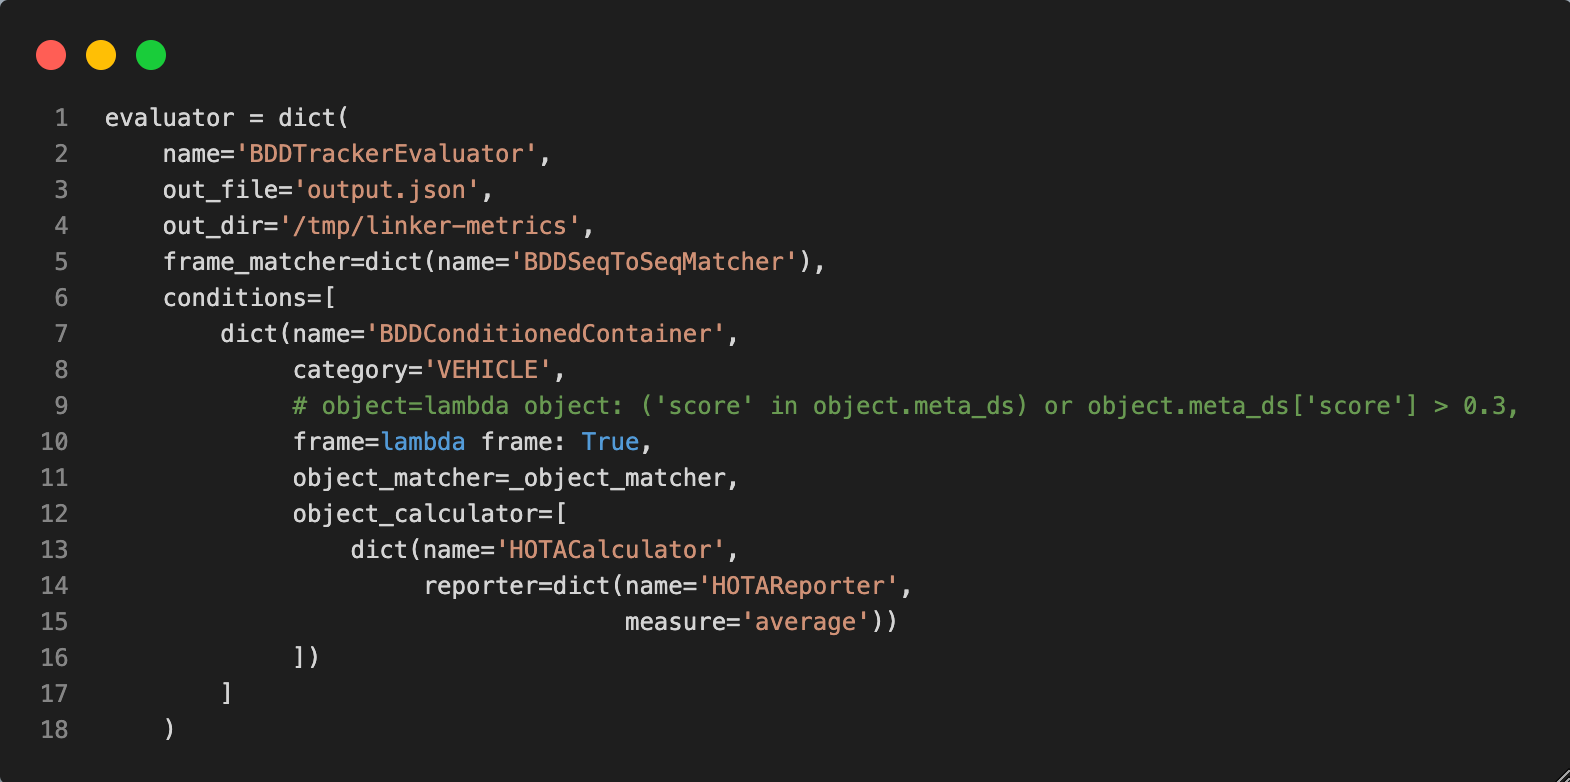
\includegraphics[width=280pt]{pics/fig13.png}
% 		\caption{linker-metrics uses config file to control the evaluation process.}
% 	\end{figure}

% \end{frame}

% \begin{frame}
% 	\frametitle{Processing in linker-metrics}
% 	\begin{figure}
% 		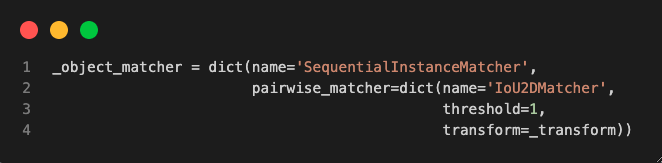
\includegraphics[width=280pt]{pics/fig14.png}
% 		\caption{The sequential instnace matcher use IoU Matcher as a pre-matcher.}
% 	\end{figure}
% \end{frame}

% \begin{frame}
% 	\frametitle{Calculation for HOTA scores}

% 	Each step in calculation of HOTA scores is performed by frame matcher, object matcher
% 	and object calculator in linker-metrics.

% 	\begin{itemize}
% 	\item The {\tt sequence-to-sequence matcher} parses the matched data sequentially.

% 	\item The object matcher {\tt sequential instances matcher} calculate the proxies
% 		during a `pre-match' performed by the build-in pre-matcher (here uses {\tt IoU matcher}).

% 	\item Then the object calculator {\tt HOTACalculator} calculate the HOTA scores
% 		according to the actual matching returned by object matcher.
% 	\end{itemize}

% \end{frame}

% \begin{frame}
% 	\frametitle{Take a Look on the Results}
% 	\begin{figure}
% 		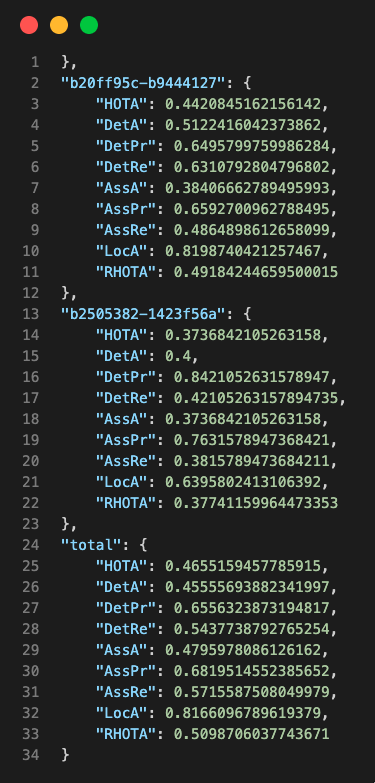
\includegraphics[height=140pt]{pics/fig15.png}
% 		\caption{HOTA in linker-metrics reports the statistics of every sequence and the result in total.}
% 	\end{figure}
% \end{frame}

% \begin{frame}
% 	\frametitle{Reference}

% 	\small

% 	\begin{itemize}
% 	\item {\tt J. Luiten, A. O\u{s}ep, P. Dendorfer, P. Torr, A. Geiger \& L. Leal-Taix\'e},
% 		\emph{HOTA: A Higher Order Metric for Evaluating Multi-object Tracking}, International Journal of Computer Vision (2021).
% 	\item {\tt R. Kasturi, et al.},
% 		\emph{Framework for Performance Evaluation of Face, Text, and Vehicle Detection and Tracking in Video:
% 		Data, Metrics, and Protocol}, IEEE Transactions on Pattern Analysis and Machine Intelligence,
% 		Vol. 31, No. 2, Feb. 2009.
% 	\end{itemize}
% \end{frame}

\end{document}